\documentclass[utf8]{beamer}
\usepackage [utf8]{inputenc}
\usepackage[russian]{babel}
\usepackage{caption}
\usepackage{cmap}
\usepackage[backend=bibtex]{biblatex}
\bibliography{DipBib}
\usepackage[T2A]{fontenc}
\usepackage{cmap}
\newsavebox{\longestsec}
\usetheme{Madrid}
\useoutertheme{tree}
\usepackage{epstopdf}
\usepackage{float}


\renewcommand{\figurename}{Fig.}

\DeclareGraphicsExtensions{.eps} 

\newtheorem{mdefinition}{Определение}[section]
\newtheorem{mremark}{Примечание}[subsection]
\newtheorem{msuggest}{Предложение}[subsection]
\newtheorem{mclaim}{Утверждение}[subsection]
\newtheorem{mlemma}{Лемма}[subsection]
\newtheorem{mtheorem}{Теорема}
\newtheorem{mconseq}{Следствие}

\DeclareMathOperator{\argmax}{argmax}
\DeclareMathOperator{\argmin}{argmin}
\DeclareMathOperator{\grad}{grad}
\DeclareMathOperator{\sign}{sign}
\DeclareMathOperator{\diag}{diag}
\DeclareMathOperator{\norm}{norm}
\renewcommand{\leq}{\leqslant}
\renewcommand{\geq}{\geqslant}
\renewcommand{\phi}{\varphi}
\setcounter{figure}{0}


\title{Сходимость ARTM}
\date{23 ноября 2016}
\author{Ирхин Илья Александрович}

\institute{
 МФТИ. ФИВТ. Кафедра анализа данных \\
    \vspace{0.7cm}
    Научный руководитель:  д.ф.-м.н. Воронцов Константин Вячеславович \\
    \vspace{0.7cm}
}

\begin{document}
	\begin{frame}
		\titlepage
	\end{frame}

	\begin{frame}
		\frametitle{Краткое содержание}
		\renewcommand{\baselinestretch}{1.5}
		\fontsize{12pt}{9.2}\selectfont
		\tableofcontents
	\end{frame}
	
	\section{Вероятностный EM алгоритм}
	\subsection{Общий вид}
	\begin{frame}	
	\frametitle{Общий вид ЕМ-алгоритма}
\textbf{Задача:} имеются наблюдаемые переменные $X$, скрытые переменные $Z$ и параметры $\Omega$. Требуется максимизировать неполное правдоподобие для какой-то вероятностной модели:
\[
\log p(X|\Omega) = \log \int\limits_Z p(D, Z|\Omega) \to \max\limits_{\Omega}
\]
В случае тематического моделирования $D$ --- это коллекция документов со словами, $Z$ --- темы для каждого вхождения слова в коллекцию, а $\Omega$ --- это $\Phi$ и $\Theta$. Так как число тем конечно, то интеграл будет превращаться в сумму.
	\end{frame}
	
	\begin{frame}	
	\frametitle{Общий вид ЕМ-алгоритма}
\[
\log p(X|\Omega) = \log \int\limits_Z p(X, Z|\Omega) \to \max\limits_{\Omega}
\]
 Пусть $q(Z)$ --- произвольное распределение на скрытых переменных:
\[
\log p(X|\Omega) = \int q(Z) \log p(X|\Omega) dZ = \int q(Z) \frac{\log p(X, Z|\Omega)}{\log p(Z|X,\Omega)} dZ = 
\]
\[
=  \int q(Z) \frac{\log p(X, Z|\Omega)}{q(Z)} \frac{q(Z)}{\log p(Z|X,\Omega)} dZ =  
\]
\[
= \underbrace{  \int q(Z) \log p(X, Z|\Omega) dZ  - \int q(Z) \log q(Z) dZ }_{F(q, \Omega)} +  \underbrace{  \int q(Z) \frac{q(Z)}{p(Z|X,\Omega)} dZ }_{KL(q(Z)\|p(Z|X,\Omega))}
\]
	\end{frame}

	
	\begin{frame}	
	\frametitle{Общий вид ЕМ-алгоритма}
\[
F(q, \Omega) + KL(q(Z)\|p(Z|X,\Omega)) \to \max\limits_{\Omega}
\]
В силу неотрицательности $KL$ слагаемое $F(q, \Omega)$ является нижней оценкой на величину $\log p(X|\Omega)$. От максимизации $\log p(X|\Omega)$ по $\Omega$ предлагается перейти к максимизации нижней границы $F(q, \Omega)$ по $q$ и $\Omega$. ЕМ-алгоритм состоит в итеративном повторении двух шагов:
\begin{enumerate}
\item $F(q, \Omega) \to \max\limits_q$
\item $F(q, \Omega) \to \max\limits_{\Omega}$
\end{enumerate}

Решением первого шага является $q(Z) = p(Z|X,\Omega)$. 

Решением второго --- $\argmax\limits_{\Omega} \mathbf{E}_{q(Z)} \log p(X, Z|\Omega)$
	\end{frame}
	
	\subsection{Введение априорного распределения}
	\begin{frame}	
	\frametitle{Введение априорного распределения}
	Вместо максимизации апостериорной вероятности $p(X|\Omega)$ максимизируется полная  вероятность $p(X, \Omega)= p(X|\Omega) p(\Omega)$. Аналогично предыдущему выводу получается:
\[
\log p(X|\Omega) + \log p(\Omega) = F(q, \Omega) + KL(q(Z)\|p(Z|X,\Omega)) + \log p(\Omega) \to \max\limits_{\Omega}
\]

\textbf{E-step}: $\argmin_{q(Z)} \left( KL(q(Z)\|p(Z|X,\Omega))\right) = p(Z|X, \Omega)$

\medskip

\textbf{М-шаг:} $\argmax_{\Omega} \left( \mathbf{E}_{q(Z)} \log p(X, Z|\Omega) + \log p(\Omega)\right)$ 
	\end{frame}


	\subsection{Тематическое моделирование}

 	\begin{frame}
		\frametitle{Дополнительные обозначения}  
$D$ --- конечное множество документов
\smallskip

$W$  --- конечное множество терминов
\smallskip

$T$ --- конечное множество тем
\smallskip

Исходные данные:
$X = (d_i ,w_i)_{i=1}^n = (w_{di})_{D \times n_d} = (n_{dw})_{D \times W}$
\smallskip

Скрытые переменные:
$Z = (d_i , t_i)_{i=1}^n = (t_{di})_{D \times n_d}$
\smallskip

Параметы модели:
$\Omega = (\Phi, \Theta)$
\smallskip

Совместная вероятность данных и скрытых переменных:
\[
p(X, Z|\Phi, \Theta) =\prod\limits_{i=1}^{n} p(w_{i}, t_{i}|\Phi, \Theta) =\prod\limits_{i=1}^{n} \phi_{w_{i}t_{i}}\theta_{t_{i}d_{i}}
\]
	\end{frame}

	
 	\begin{frame}
		\frametitle{Вероятностный вывод PLSA. Е-шаг}   
На E-шаге необходимо оценить распределение на скрытых переменных при условии параметров и  наблюдаемых величин: $p(Z|D,\Phi,\Theta)$. Так как словопозиции независимы, то сразу можно перейти к отдельным вероятностям:
\[
p(Z|D,\Phi, \Theta) = \prod\limits_{i=1}^{n} \phi_{w_{i}t_{i}}\theta_{t_{i}d_{i}}
\]

Чтобы найти эти вероятности, воспользуемся формулой Байеса:
\[
p(t_{i}|w_{i}, \Phi, \Theta) = \frac{p(w_{i}|t_{i}, \Phi, \Theta)p(t_{i}|\Phi,\Theta)}{\sum_{t=1}^T p(w_{i}|t, \Phi, \Theta)p(t|\Phi,\Theta)}
= \frac{\phi_{w_{i} t_{i}} \theta_{t_{i} d_i}}{\sum_{t=1}^T \phi_{w_{i}t} \theta_{td_i}}
\]
Фактически, это знакомые нам $p_{tdw}$.
	\end{frame}
	
	 	\begin{frame}
		\frametitle{Вероятностный вывод PLSA. М-шаг}   
\[
\mathbf{E}_{p(Z|D,\Phi, \Theta)} \log p(D,Z|\Phi,\Theta) = 
\sum_{i=1}^{n} \mathbf{E}_{p(t|w_{i}, d_{i}, \Phi, \Theta)} (\log \phi_{w_{i} t_{i}} + \log \theta_{t_{i} d_{i}}) =
\]
\[
= \sum_{i=1}^{n} \sum_{t \in T} p(t_{i}=t|w_{i}, d_{i},\Phi,\Theta) (\log \phi_{w_{i} t} + \log \theta_{td_{i}}) =
\]
\[
= \sum_{i=1}^{n} \sum_{t \in T} p_{td_{i}w_{i}} (\log \phi_{w_{i} t} + \log \theta_{td_i}) =
\]
\[
=\sum_{d\in D}\sum_{w \in W} \sum_{t \in T} n_{dw} p_{tdw} (\log \phi_{wt} + \log \theta_{td}) = Q(\phi, \theta)
\]
На каждом М-шаге нужно максимизировать данный функционал или хотя бы не уменьшать.
	\end{frame}
	
	\begin{frame}
	\frametitle{Вероятностный вывод ARTM}
	Регуляризатор $R$ можно интерпретировать как $\log p(\Omega)$, поскольку, формально, для вывода не нужна вероятностная природа для $p(\Omega)$, это лишь дополнительное слагаемое для оптимизации на М-шаге.
	\medskip
	
	\textbf{E-шаг:}	
   		 
   		 \qquad $p_{tdw} = p(t|d, w) = \frac{\phi_{wt} \theta_{td}}{\sum\limits_{s\in T} \phi_{ws} \theta_{sd}}$ 		 
 		\medskip
 		
 	\textbf{M-шаг:}
 	
   		 
   		 \qquad $\sum\limits_{d\in D}\sum\limits_{w \in W} \sum\limits_{t \in T} n_{dw} p_{tdw} (\log \phi_{wt} + \log \theta_{td})  + R(\phi,\theta) \to \max\limits_{\phi,\theta}$
   	\medskip
   		 
	При произвольном $R$ задачу М-шага невозможно решить точно. Но можно, используя разные эвристики, увеличивать значения данного функционала. Это будет GEM алгоритм.
	\end{frame}
	
 	\begin{frame}
		\frametitle{Формулы ARTM}   
		Применим теорему Каруша-Куна-Таккера к функционалу М-шага. В качестве точки увеличения будем брать итерирование этой системы уравнений один раз. Получаем известные нам формулы ARTM:
		\medskip
		
   		\textbf{E-шаг:}	
   		 
   		 \qquad $p_{tdw} = p(t|d, w) = \norm_t(\varphi_{wt} \theta_{td})$ 		 
 		\medskip
 		
 		\textbf{M-шаг:}
    
 		\qquad $n_{wt} = \sum\limits_{d} n_{dw} p_{tdw}$,\ \ \ $r_{wt} =  \phi_{wt}\dfrac{\partial R}{\partial\phi_{wt}}$,\ \ \  $\phi_{wt}   = \norm_w\big(n_{wt} + r_{wt}\big)$,

 		\qquad $n_{td} = \sum\limits_{w} n_{dw} p_{tdw}$,\ \ \  \ $r_{td} =  \theta_{td}\dfrac{\partial R}{\partial\theta_{td}}$,\ \ \ \ \ $\theta_{td} = \norm_t  \big(n_{td} + r_{td}\big)$,
\medskip

	где $norm_y(x) = \frac{(x)_{+}}{\sum\limits_y (x)_{+}}$, и $(x)_{+} = \max(x, 0)$. $r_{wt}$ и $r_{td}$ называются регуляризационными поправками. 
	\end{frame}


	\section{Сходимость алгоритма ARTM}
	\subsection{Теорема о сходимости}
	
\begin{frame}
\frametitle{Теорема о сходимости}
\footnotesize{
Под $x^k$ понимается значение $x$ на $k$-ой итерации. 

Пусть выполнены следующие условия:
\begin{enumerate}
\item  $ n^k_{wt} = 0 \Rightarrow \phi^k_{wt} = 0$ --- сохранение нуля.
\item $n^k_{td} = 0 \Rightarrow \theta^k_{td} = 0$ --- сохранение нуля.
\item $\exists \varepsilon>0\ \exists N\ \forall k > N\ \phi^k_{wt}, \theta^k_{td} \notin (0, \varepsilon)$ -- отделимость от нуля.
\item  $ n_{dw}>0 \Rightarrow \forall k\ \exists t\colon p^k_{tdw} > 0$ --- невырожденность распределения $ p(t|d,w)$.
\item $\exists \delta\geq 0\ \exists N\ \forall k > N \ \forall t\ \exists w\  n^k_{wt} + r^k_{wt} > \delta$ --- невырожденность $p(w|t)$.
\item $\exists \delta\geq 0\ \exists N\ \forall k > N \ \forall d\ \exists t\  n^k_{td} + r^k_{td} > \delta$ --- невырожденность $p(t|d)$.
\item $\exists N\ \forall k > N\colon\ \ Q^k (\phi^k, \theta^k)+ R(\phi^k, \theta^k) \geq Q^k(\phi^{k-1}, \theta^{k-1}) + R(\phi^{k-1}, \theta^{k-1})$, где $Q^k(\phi, \theta) = \sum\limits_{t,d,w} p^k_{tdw} (\ln \phi_{wt} + \ln \theta_{td})$ ---  монотонное неубывание нижней оценки правдоподобия.
\end{enumerate}
Тогда выполнено:
\[
KL(p_{tdw}^{k}||p_{tdw}^{k + 1}) \to 0 \text{ при } k \to \infty.
\]
\[
L(\phi^k, \theta^k) + R(\phi^k, \theta^k) \text{ монотонно сходится при } k \to \infty.
\]
}
\end{frame}

\begin{frame}
\frametitle{Несколько следствий}
\begin{enumerate}
\item  Если в условии №5 и №6 $\delta > 0$, то $\phi^k_{wt} - \phi_{wt}^{k-1} \to 0$ и $\theta^k_{td} - \theta^{k-1}_{td} \to 0$.
\item Все предельные точки $\phi^k_{wt}$ и $\theta^k_{td}$ -- стационарные точки $L + R$ при некотором ограничении на множество нулевых позиций $\Phi$ и $\Theta$.
\item Если множество стационарных точек $L + R$ дискретно при любом ограничении на множество нулевых позиций $\Phi$ и $\Theta$, то $\phi_{wt}^k$ и $\theta_{td}^k$ сходятся к стационарной точке $L+R$ при некотором ограничении  на множество нулевых ячеек матриц $\Phi$ и $\Theta$.
\item Условия №1 -- №6 проверяются аналитически или гарантируются при реализации. Наибольшую важность играет условие №7, его сложнее всего обеспечить, так как наши методы увеличения функционала $Q$ на М-шаге эвристические.
\end{enumerate}
\end{frame}

	
\subsection{Рецепты для 'улучшения' сходимости}

\begin{frame}
\frametitle{Точка подсчёта регуляризационных поправок}
ARTM на М-шаге итерирует систему уравнений для стационарных точек максимизируемого функционала. Однако, преобразование можно применять к различным точкам. Нужно выбрать в какой точке считать регуляризационные поправки и как именно их считать:
\medskip

\begin{enumerate}
\item Оригинальный способ. Брать $\phi$ и $\theta$ с предыдущей итерации.
\item Несмещённая модификация. Брать $\frac{n_{wt}}{n_t}$ и $ \frac{n_{td}}{n_d}$ вместо $\phi_{wt}$ и $\theta_{td}$ соответственно.
\item Градиентная модификация. Брать $\frac{\partial{R}}{\partial{n_{wt}}} $ и $ \frac{\partial{R}}{\partial{n_{td}}}$ в качестве $r_{wt}$ и $r_{td}$ соответственно.
\item Использовать частичное применение регуляризаторов. Об этом немного позже.
\end{enumerate}
\end{frame}
	
	
\begin{frame}
\frametitle{Обоснование формул}
Градиент $R$ по $n_{wt}$ и $n_{td}$ равен:
\[
\frac{\partial{R}}{\partial{n_{wt}}} = \frac{1}{n_t} \bigg(\frac{\partial{R}}{\partial{\phi_{wt}}} - \sum\limits_u \phi_{ut} \frac{\partial{R}}{\partial{\phi_{ut}}}\bigg),
\]
\[
\frac{\partial{R}}{\partial{n_{td}}} = \frac{1}{n_d} \bigg( \frac{\partial{R}}{\partial{\theta_{td}}} - \sum\limits_s \theta_{sd} \frac{\partial{R}}{\partial{\theta_{sd}}} \bigg).
\]
Для несмещённой модификации угол между вектором изменений $\Delta n_{wt}, \Delta n_{td}$ и данным градиентом всегда острый, что гарантирует локальное увеличение $R$. Однако, наибольшее локальное увеличение даёт именно изменение вдоль градиента.
\end{frame}


\begin{frame}
\frametitle{Несмещённая модификация}
Все вхождения $\phi_{wt}$ и $\theta_{td}$ в формулы регуляризационных поправок заменяются на их несмещённые оценки $\frac{n_{wt}}{n_t}$ и $\frac{n_{td}}{n_d}$:
\[
\left\{
	\begin{aligned}
		r_{wt} =  \frac{n_{wt}}{n_t} \frac{\partial{R}}{\partial{\phi_{wt}}} \bigg(\frac{n_{wt}}{n_t}, \frac{n_{td}}{n_d}\bigg),\\
		r_{td} = \frac{n_{td}}{n_d} \frac{\partial{R}}{\partial{\theta_{td}}} \bigg(\frac{n_{wt}}{n_t}, \frac{n_{td}}{n_d}\bigg).
	\end{aligned}
\right.
\]
\end{frame}

	
\begin{frame}
\frametitle{Градиентная модификация}
Для улучшения сходимости предлагается использовать градиент регуляризатора в формуле М-шага.
\[
\left\{\
	\begin{aligned}
		r_{wt} =  A_t \bigg[\textcolor{red} {\frac{\partial{R}}{\partial{\phi_{wt}}} - \sum\limits_u \phi_{ut} \frac{\partial{R}}{\partial{\phi_{ut}}} }\bigg] \bigg(\frac{n_{wt}}{n_t}, \frac{n_{td}}{n_d}\bigg),\\
		r_{td} =  B_d \bigg[ \textcolor{red} {\frac{\partial{R}}{\partial{\theta_{td}}} - \sum\limits_s \theta_{sd} \frac{\partial{R}}{\partial{\theta_{sd}}} }\bigg] \bigg(\frac{n_{wt}}{n_t}, \frac{n_{td}}{n_d}\bigg),
	\end{aligned}
\right.
\]
Где $A_t$ и $B_d$ -- коэффициенты, зависящие только от темы(документа). Эту добавку можно эффективно вычислить, поскольку второе слагаемое одинаковое для всех слов (тем) в рамках одной темы (документа).
\end{frame}



\begin{frame}
\frametitle{Более подробно про острый угол градиента}

Для упрощения будет рассмотрен случай $R(\Phi, \Theta) = R(\Phi)$.
\[
\frac{\partial{R}}{\partial{n_{wt}}}  = \frac{1}{n_t} \sum_{u} \bigg(\frac{\partial{R}}{\partial{\phi_{wt}}}  -  \frac{\partial{R}}{\partial{\phi_{ut}}} \bigg)  \phi_{ut}.
\]
С другой стороны изменение $n_{wt}$ на итерации равно $ \Delta n_{wt} =  \phi_{wt} \frac{\partial{R}}{\partial{\phi_{wt}}}$.
\[
(\overline{\Delta n_{wt}}, grad\ R(n_{wt}, n_{td})) = \sum\limits_{w, t, u}  \frac{1}{n_{t}}  \bigg(  \frac{\partial{R}}{\partial{\phi_{wt}}}  -  \frac{\partial{R}}{\partial{\phi_{ut}}}  \bigg)  \frac{\partial{R}}{\partial{\phi_{wt}}} \phi_{wt} \phi_{ut}  = 
\]
\[
= \frac12  \sum\limits_{t, w, u}  \frac{1}{n_{t}} \bigg(  \frac{\partial{R}}{\partial{\phi_{wt}}}  -  \frac{\partial{R}}{\partial{\phi_{ut}}}  \bigg)^2 \phi_{wt} \phi_{ut}  \geq 0.
\]
\end{frame}

\begin{frame}
\frametitle{Частичное применение регуляризаторов}
Для некоторых регуляризаторов возможно явно найти решение  задачи  максимизации  $Q$ на М-шаге, например, регуляризаторы сглаживания и разреживания. Такие регуляризаторы нназовём аналитическими.
\medskip

Пусть $R = R_1 + R_2$, где $R_1$ --- аналитический регуляризатор. На М-шаге необходимо построить увеличение функционала $Q + R = Q + R_1 + R_2$. По формулам М-шага вычисляется $(n_{wt}$, $n_{td})$ как точка максимума $Q$, а затем увеличивается $R$.  
\medskip

Однако, можно определить $(n_{wt},n_{td})$ как точку максимума $Q + \tau R_1 $ (это можно сделать в силу аналитичности $R_1$), а затем производить увеличение $R_2$. Таким образом,  численные методы оптимизации будут использоваться только для той части регуляризатора, где не получается явно найти максимум.
\end{frame}

\section{Эксперимент}
\subsection{Описание эксперимента}
	
\begin{frame}
\frametitle{Эксперимент}
		
\begin{enumerate}
\item В качестве регуляризатора был взят регуляризатор декоррелирования ($R = -\tau\sum\limits_w \sum\limits_{t \neq s} \phi_{wt} \phi_{ws}$).
\item Были проверены четыре случая величины $\tau$: $10^5,~10^6,~10^7,~10^8$, для разного числа тем: 3, 10, 30.
\item Использовались статьи со спортивного сайта sports.ru по 7 видам спорта.
\item Проверялись стандартная формула, замена несмещёнными оценками и градиентное преобразование.
\item Алгоритм  запускался из случайных начальных приближений, одинаковых для всех запусков, после чего сравнивались средние значения целевых метрик.
\end{enumerate}
\end{frame}

\subsection{Полученые результаты}
\captionsetup{labelformat=simple} 
\begin{frame}
\begin{figure}[h]
	\centering  	
	\caption{Значения $L + R$. $|T| = 10$. Градиентная модификация немного хуже остальных. При большом $\tau$ показывает принципиально отличный результат.} 
	\medskip
	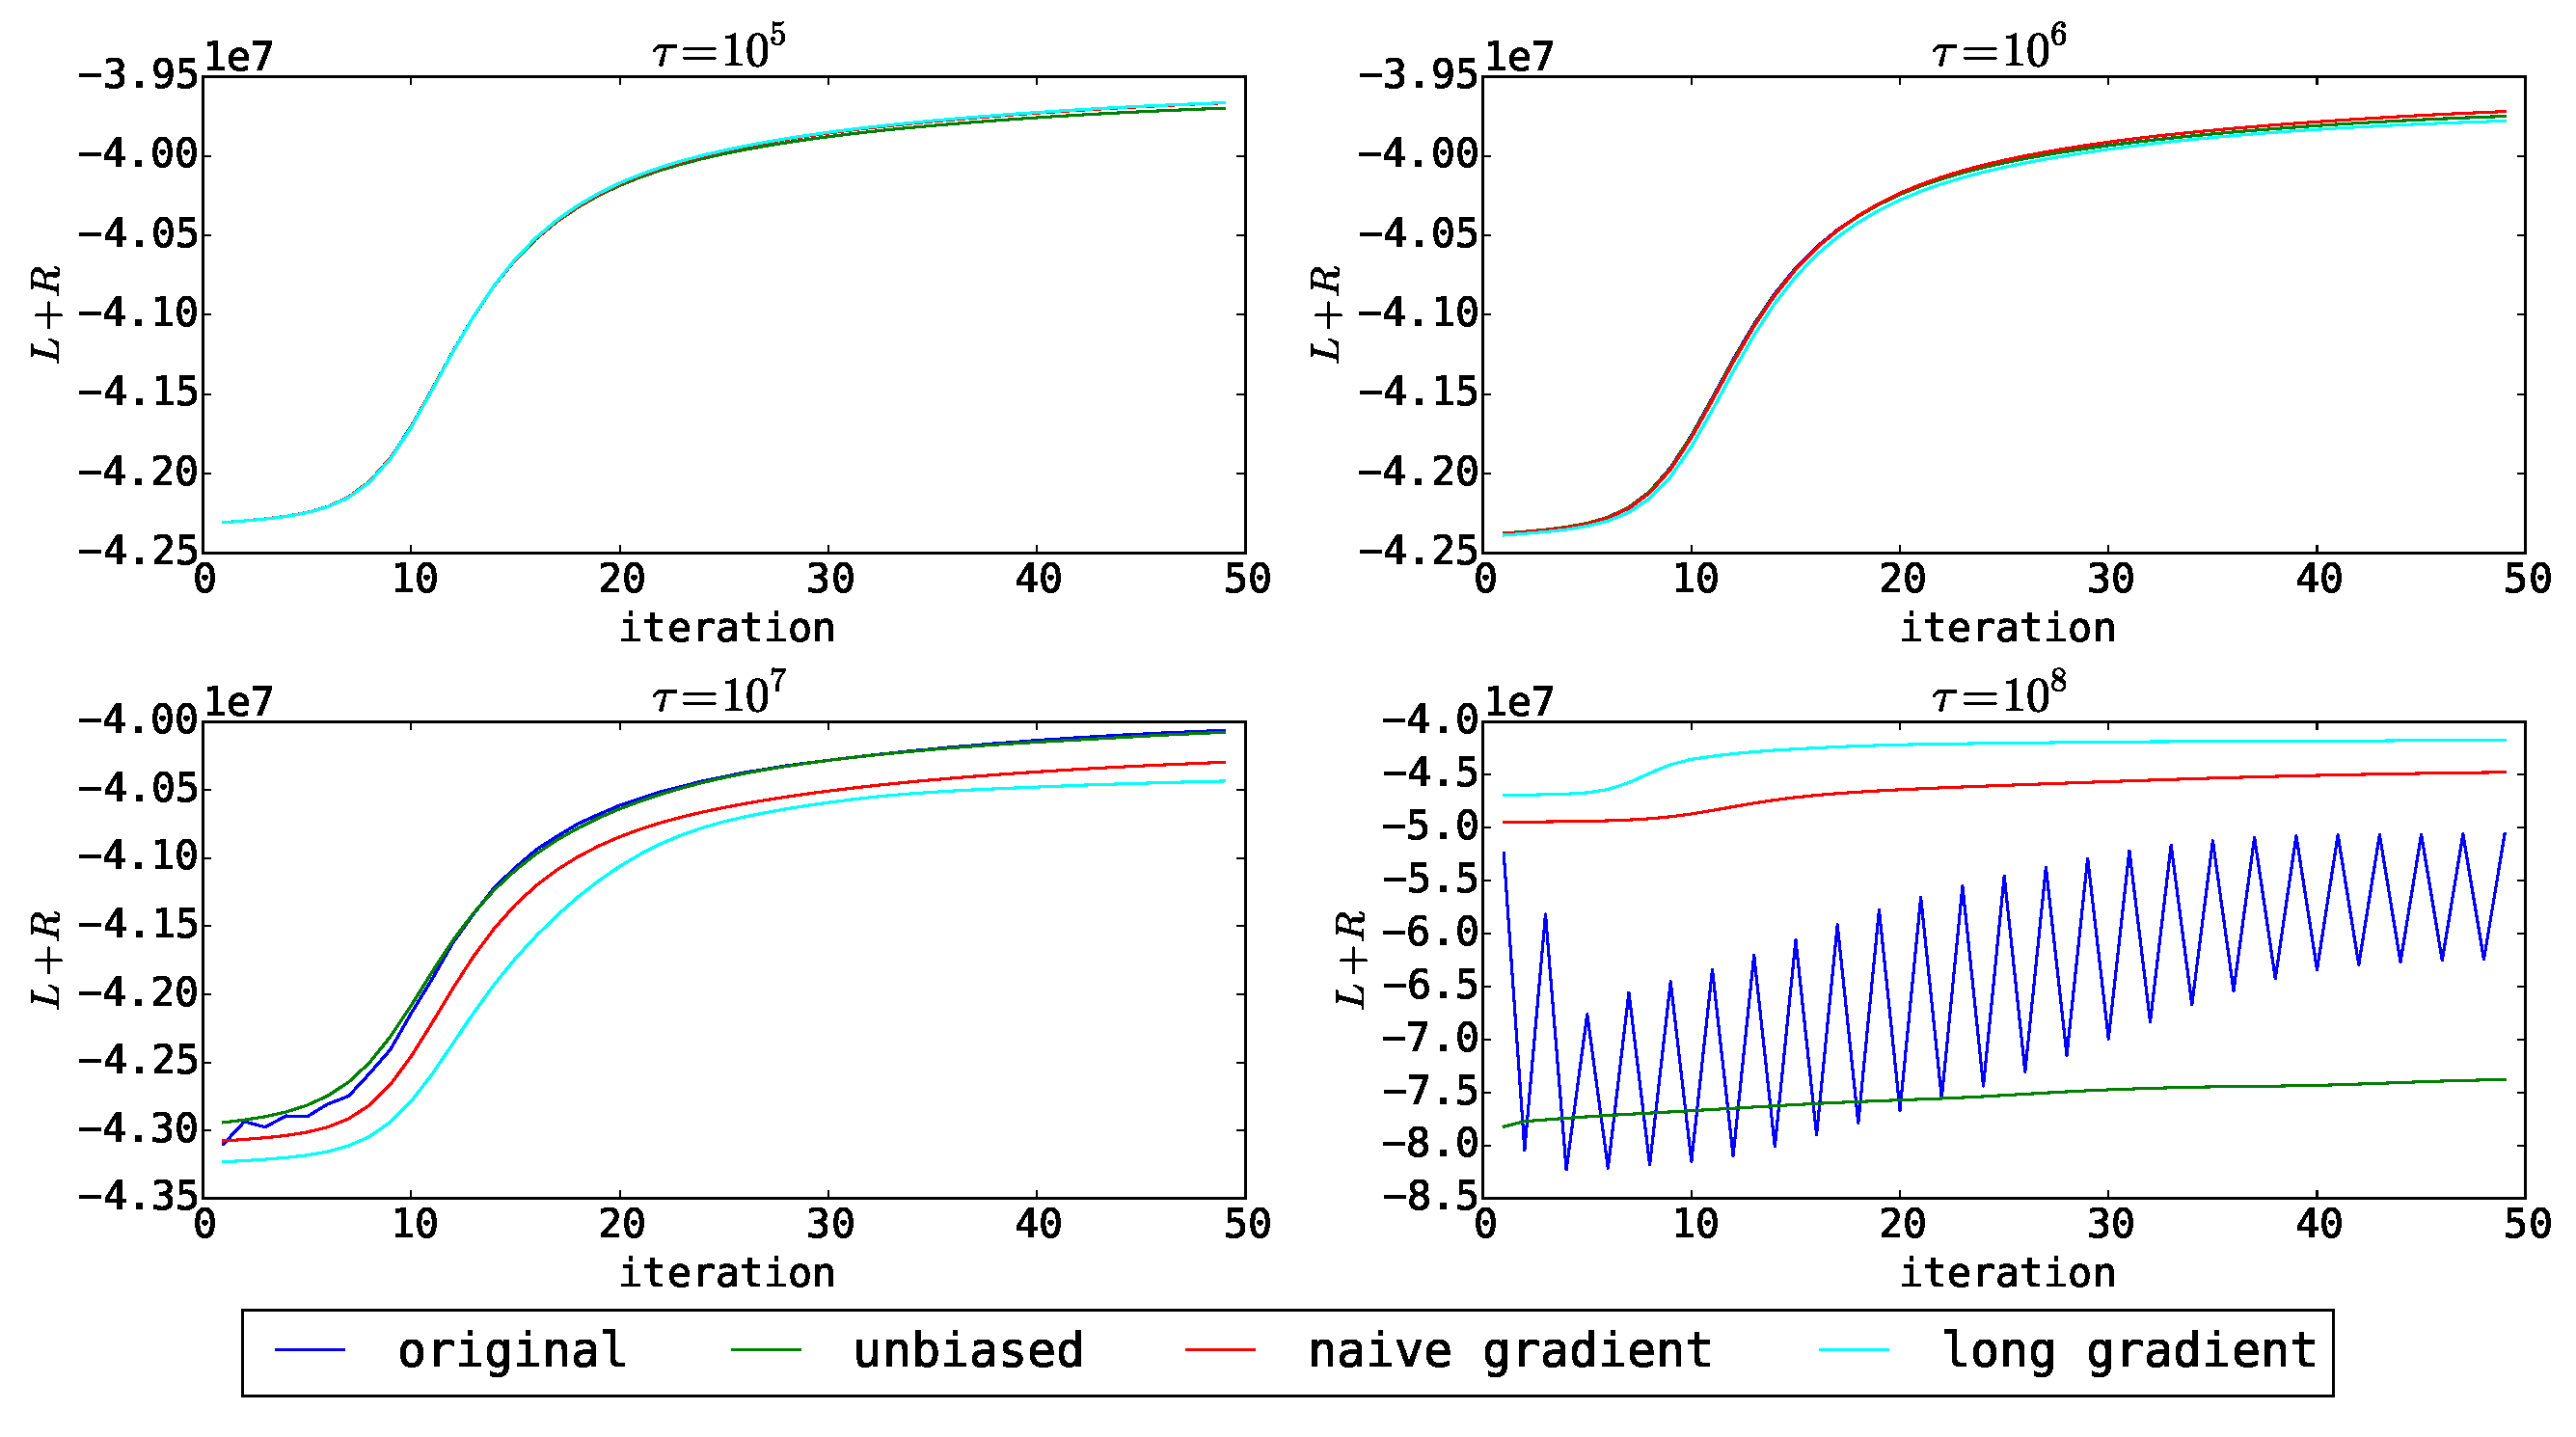
\includegraphics[width=0.9\linewidth]{presentation_pictures/topics_10_LR_values.eps}  
\end{figure}
\end{frame}

\begin{frame}
\begin{figure}[h]
	\centering   
	\caption{Значения $R$. $|T| = 10$.  На верхних графиках виден скачок $R$ на первой итераций, на нижних графиках он ярче выражен. Несмещённая модификация и длинный  градиент лучше всех остальных.} 
	\medskip
	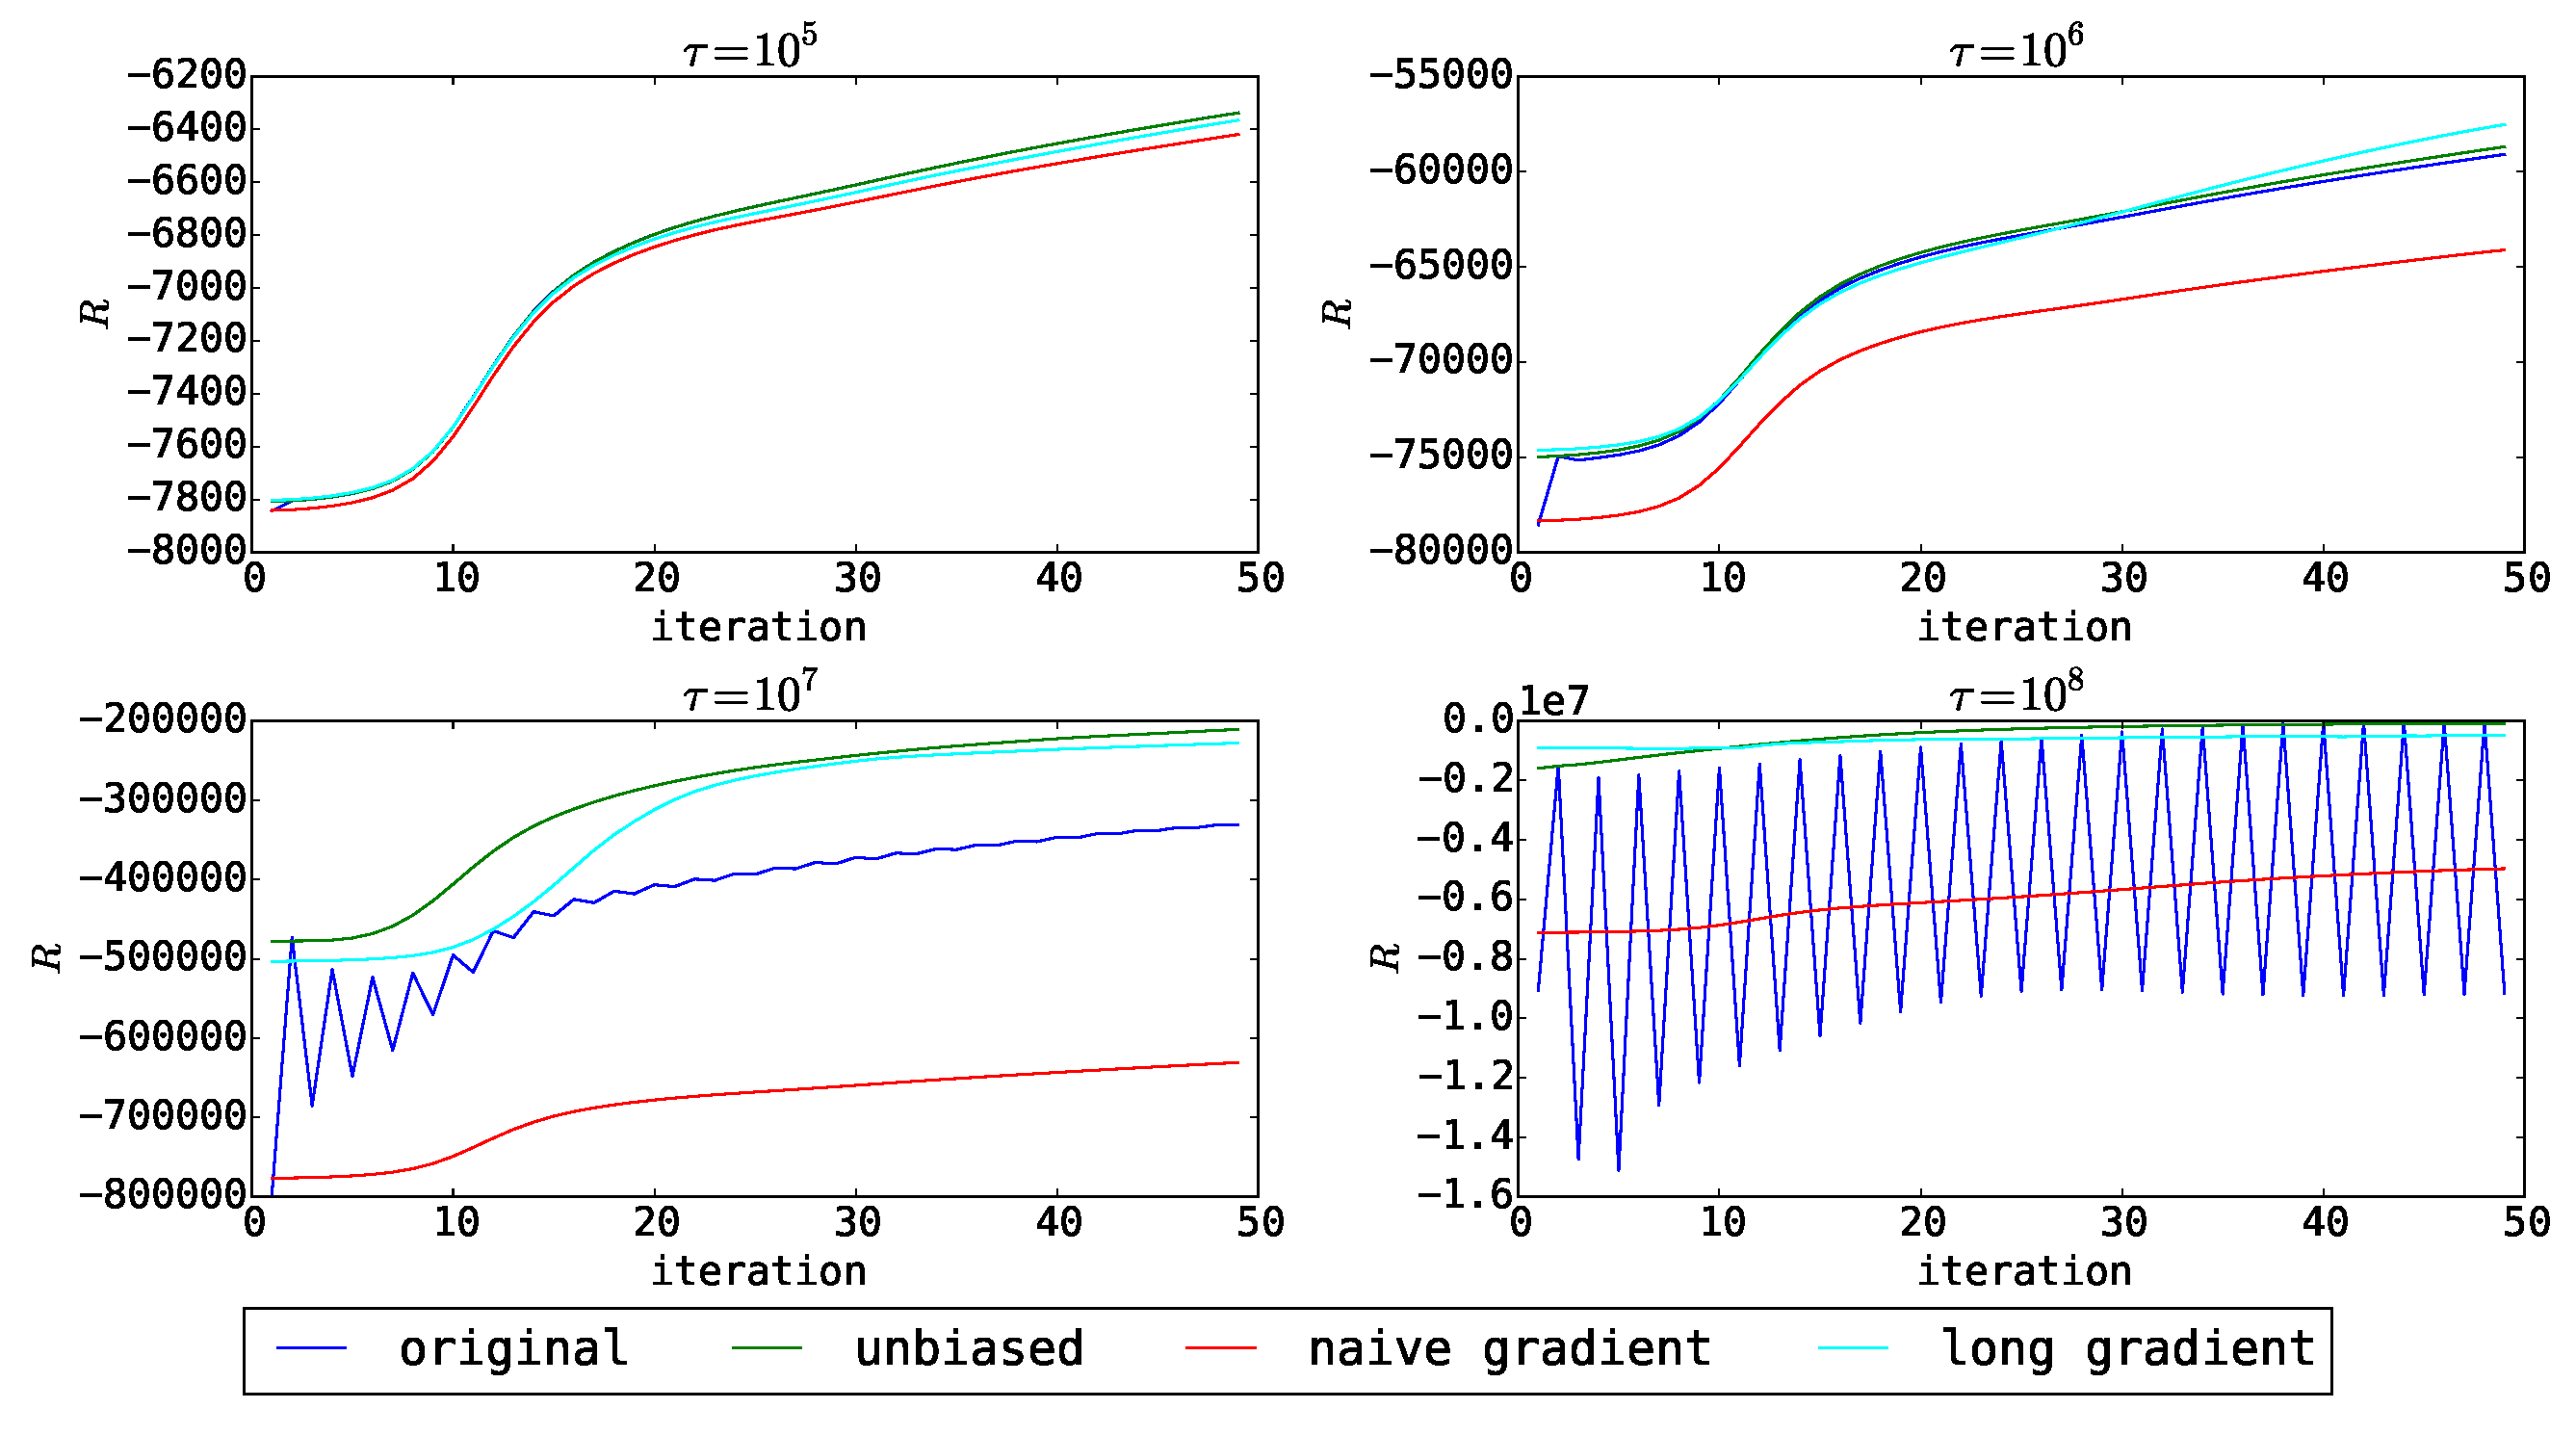
\includegraphics[width=0.9\linewidth]{presentation_pictures/topics_10_R_values.eps}  
\end{figure}
\end{frame}
	
\begin{frame}
\begin{figure}[h]
	\centering   
	\caption{Значения $R$. $|T| = 30$. Эффект скачков уже ярко выражен при $\tau = 10^6$. Длинный градиент существенно лучше всех остальных.} 
	\medskip
	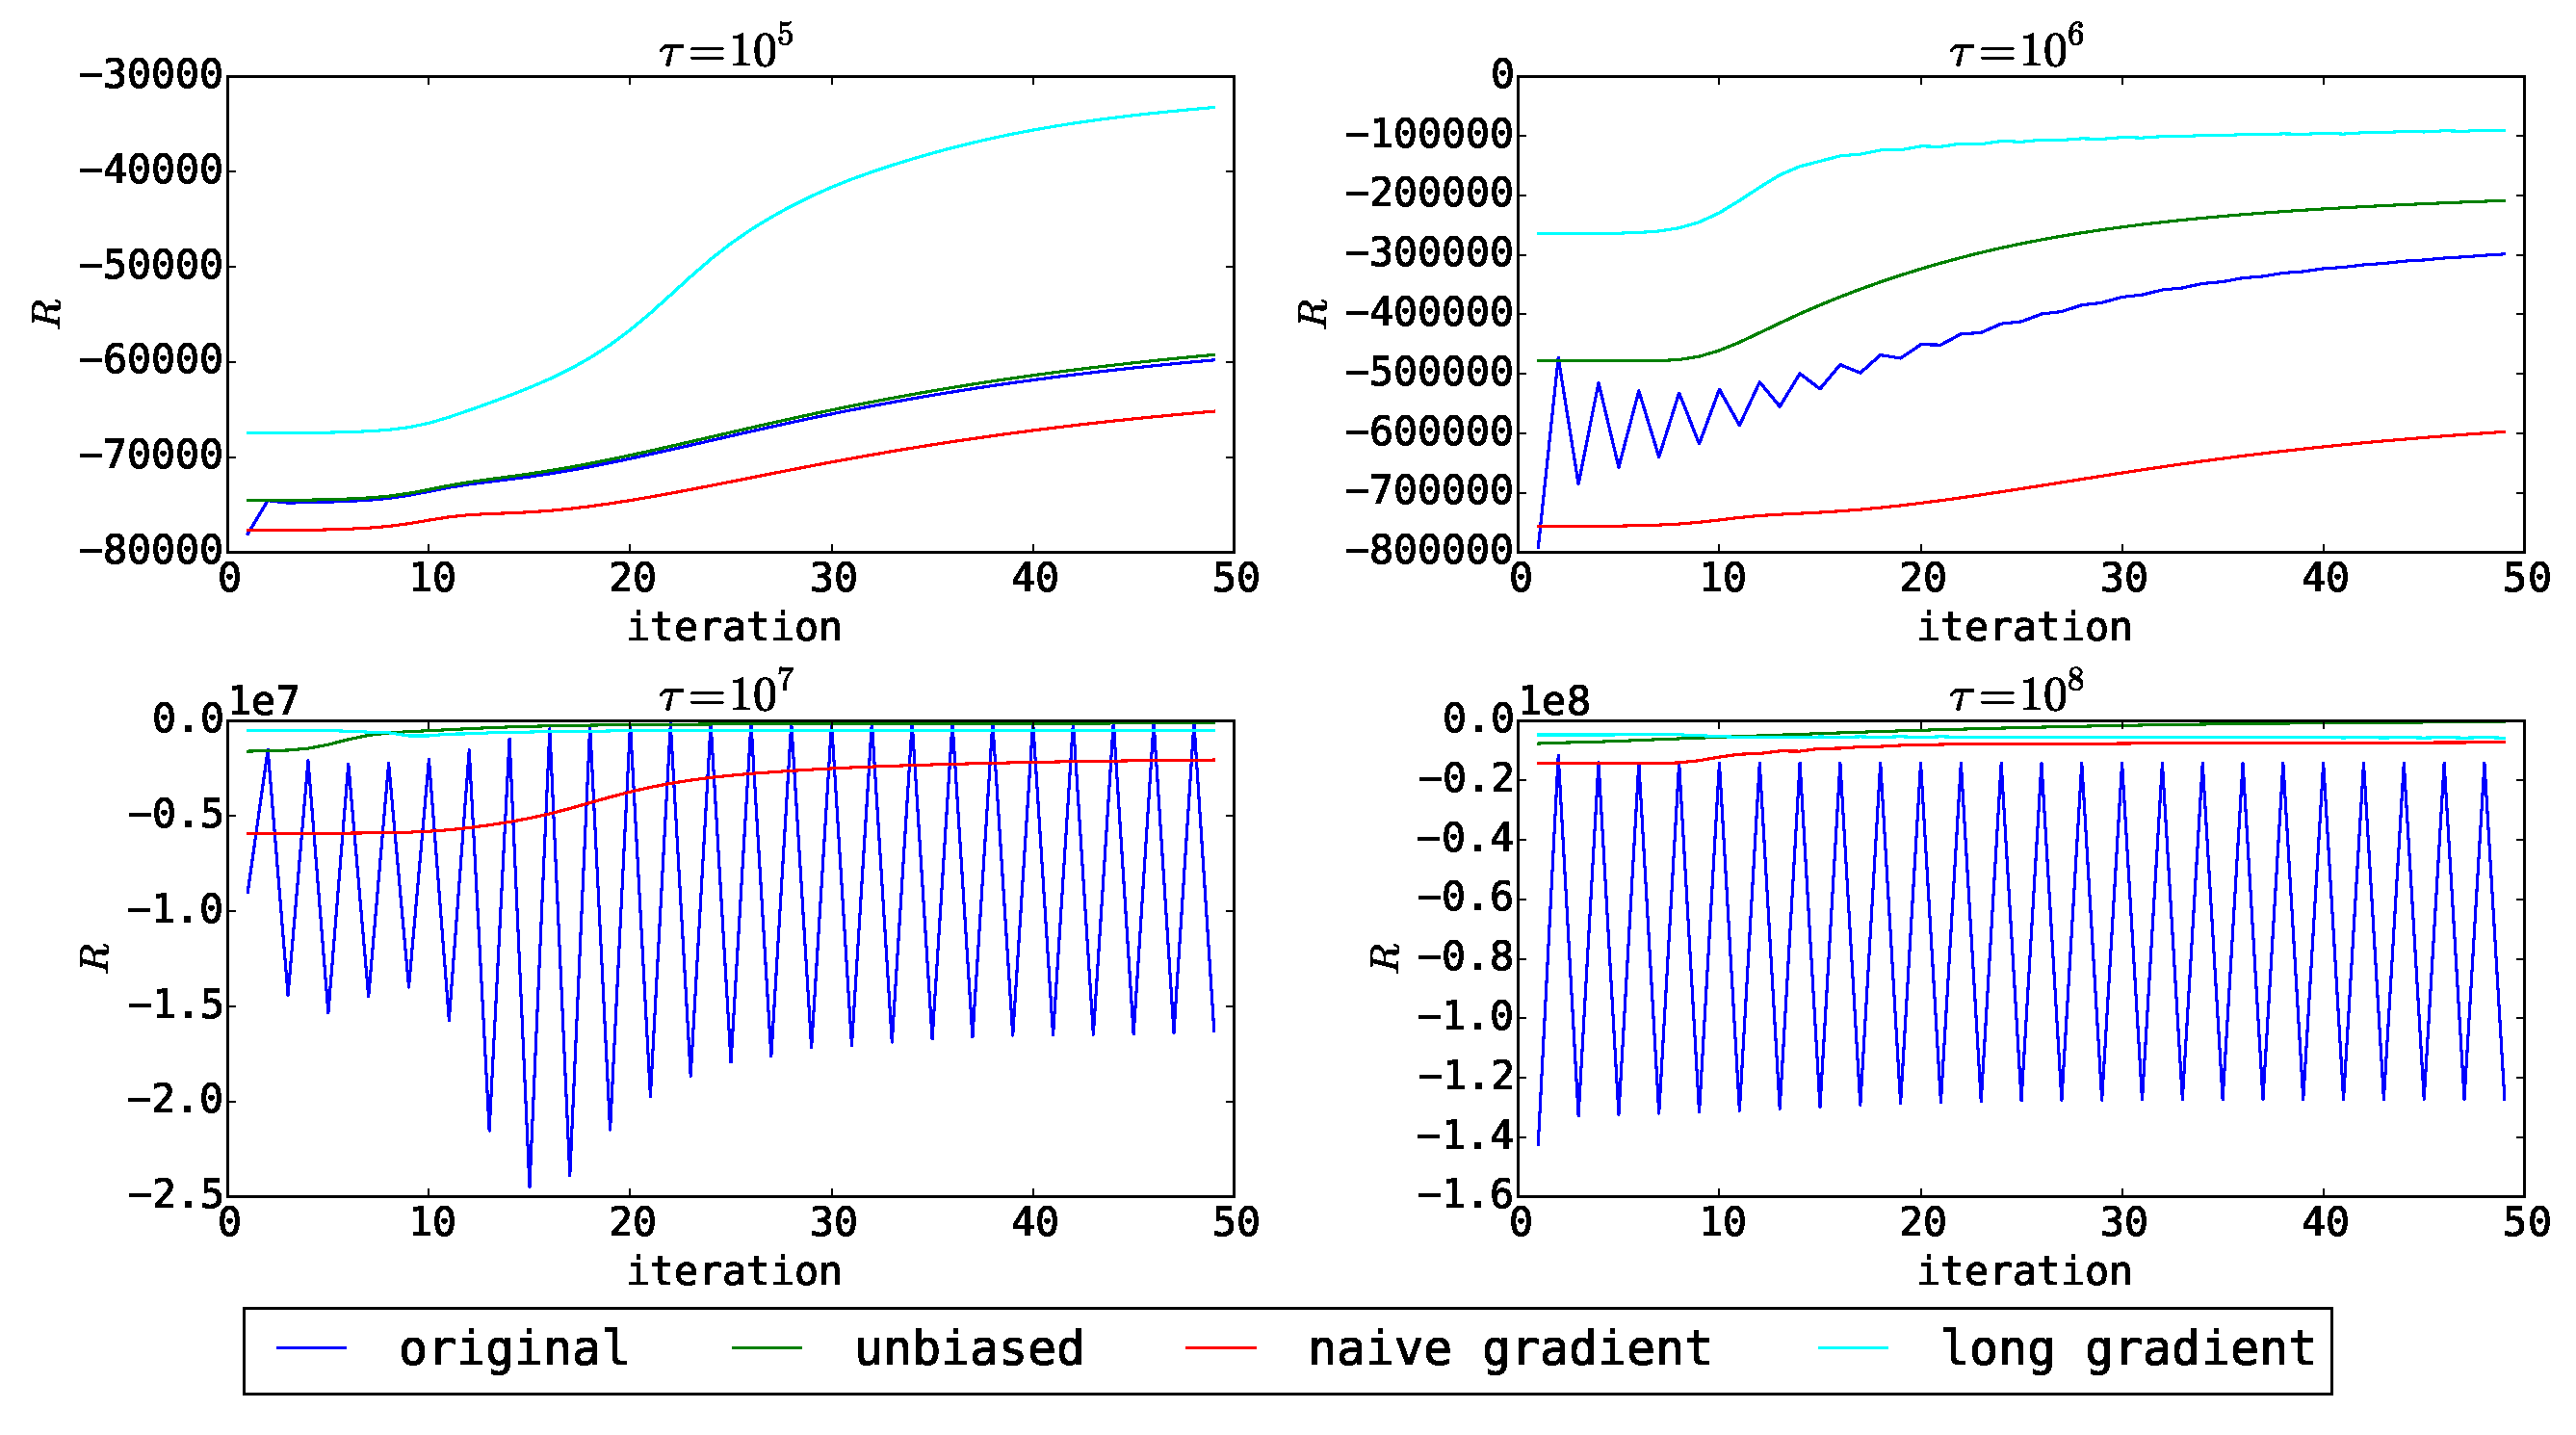
\includegraphics[width=0.9\linewidth]{presentation_pictures/topics_30_R_values.eps}  
\end{figure}
\end{frame}
	
\begin{frame}
\begin{figure}[h]
	\centering
	\caption{Логарифм минимального ненулевого значения матрицы $\Phi$. $|T| = 10$.}    
	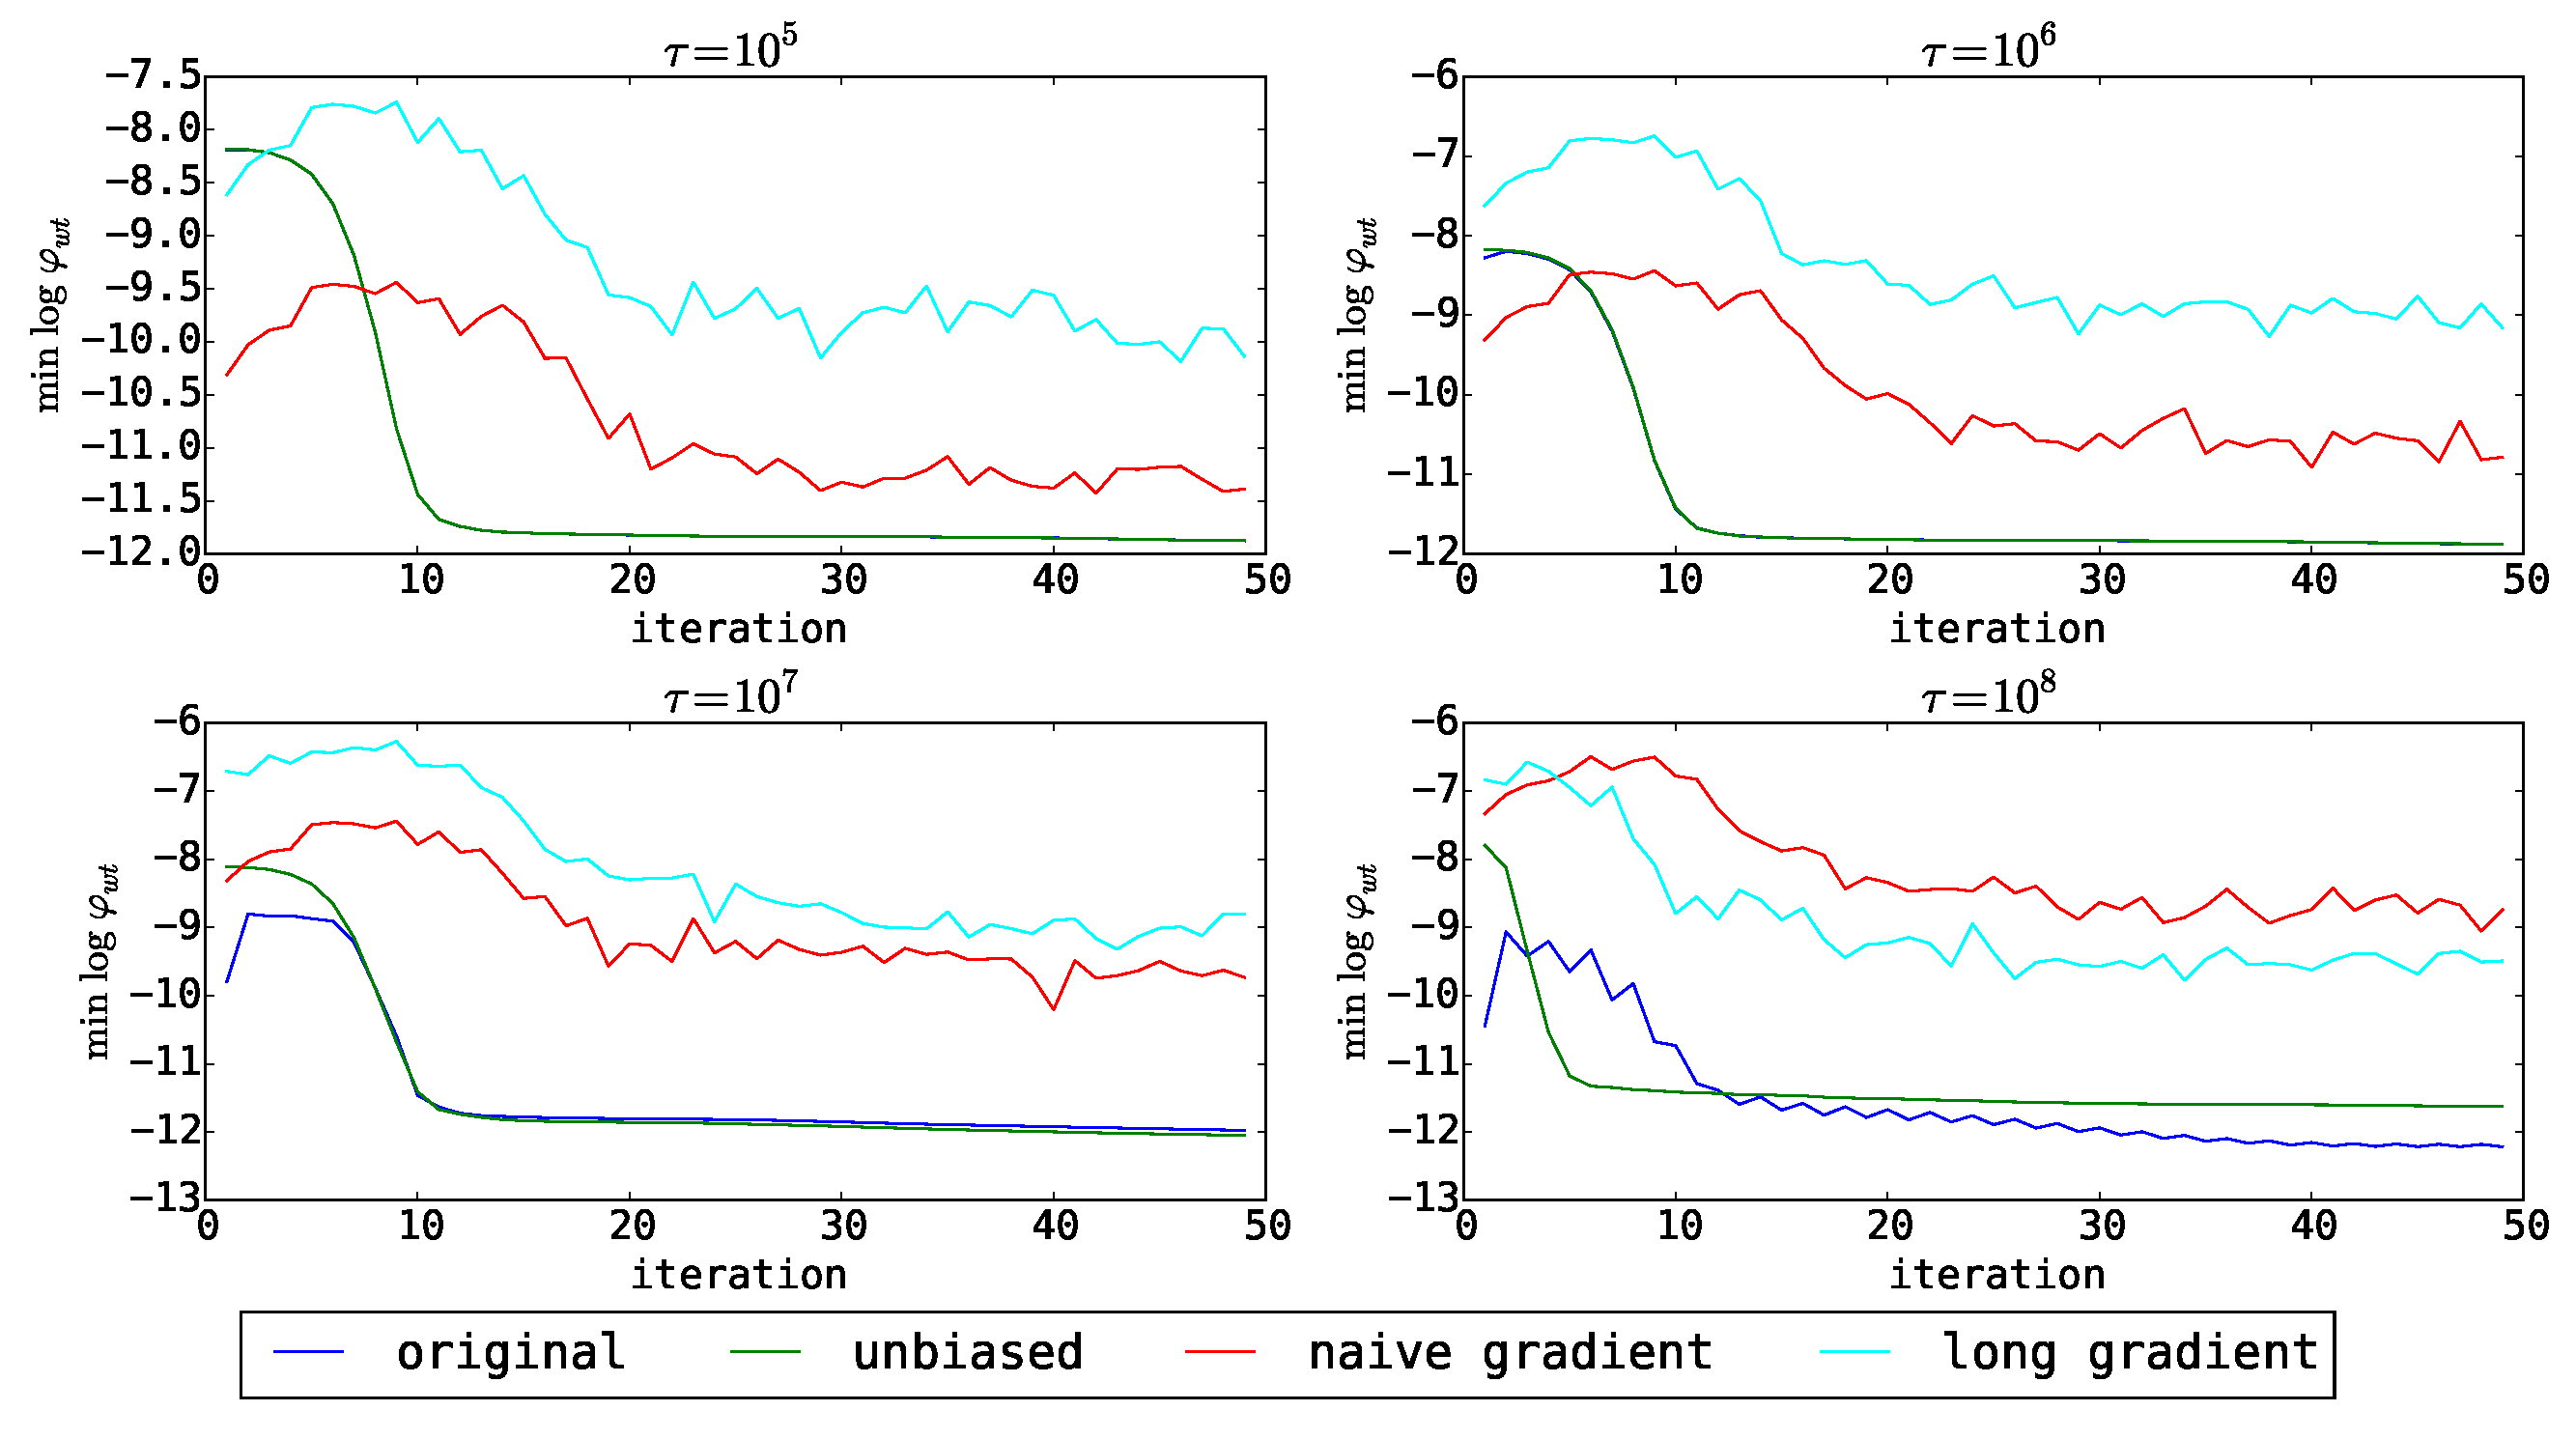
\includegraphics[width=1.0\linewidth]{presentation_pictures/topics_10_minPhi_values}
\end{figure}
\end{frame}
	
	
\begin{frame}{Итоги экспериментов}
\begin{enumerate}
\item Предположения об отделимости и невырожденности распределений выполняются на практике.
\item С точки зрения оптимизации $L +  R$ все рассмотренные формулы отличаются незначительно. Основное достоинтсво предложенных модификаций --- это теоретические гарантии и более эффективная оптимизация $R$.
\item Есть эффект скачков значений функционалов на первых итерациях для стандартной формулы, вызванный выбором точки в которой считаются $r_{wt}$ и $r_{td}$.
\item Для градиентных поправок необходимо дополнительное исследование, чтобы понять как подбирать константу перед градиентом.
\end{enumerate}
\end{frame}

\end{document}
